% article example for classicthesis.sty
\documentclass[10pt,a4paper]{article} % KOMA-Script article scrartcl
\usepackage{import}
\usepackage{xifthen}
\usepackage{pdfpages}
\usepackage{transparent}
\newcommand{\incfig}[1]{%
    \def\svgwidth{\columnwidth}
    \import{./figures/}{#1.pdf_tex}
}
\usepackage{lipsum}     %lorem ipsum text
\usepackage{titlesec}   %Section settings
\usepackage{titling}    %Title settings
\usepackage[margin=10em]{geometry}  %Adjusting margins
\usepackage{setspace}
\usepackage{listings}
\usepackage{amsmath}    %Display equations options
\usepackage{amssymb}    %More symbols
\usepackage{xcolor}     %Color settings
\usepackage{pagecolor}
\usepackage{mdframed}
\usepackage[spanish]{babel}
\usepackage[utf8]{inputenc}
\usepackage{longtable}
\usepackage{multicol}
\usepackage{graphicx}
\graphicspath{ {./Images/} }
\setlength{\columnsep}{1cm}

% ====| color de la pagina y del fondo |==== %
\pagecolor{white}
\color{black}



\begin{document}
    %========================{TITLE}====================%
    \title{\rmfamily\normalfont\spacedallcaps{ Abstract }}
    \author{\spacedlowsmallcaps{Rodrigo Castillo}}
    \date{\today}

    \maketitle


    %=======================NOTES GOES HERE===================%
    \section{Resumen del proyecto}
        En mi grupo, optamos por hacer un sistema de riego hidropónico
        automatizado según las necesidades de la planta que vayamos a sembrar.
        \\ Para esto, propusimos una idea básica la cuál vamos a ir escalando
        con respecto al proyecto:
        \subsection{Idea básica:}
            El lo primero que dispondrá el proyecto, será de un sistema de
            riego hidropónico que monitoree y controle el estado de la planta
            según 3 condiciones: el ph del agua, la humedad de la tierra y la
            cantidad de luz que las plantas estén recibiendo, para eso, será
            necesario programar un sensor de luz, un sensor de ph en el agua y
            un sensor de humedad en la tierra de cada planta, también será
            necesario programar unas lámparas con respecto a la luz necesaria
            para la planta.
            \begin{itemize}
            \item {El proyecto , en su versión básica, solamente contará con un
            tipo de planta, en el grupo aún no se ha decidido esto.

            \item {El sistema de riegos también contará con una interfaz web, la
            cuál le permitirá al usuario ver el estado de sus plantas y
            recibirá alertas en caso de que alguno de los sensores detecte que
            necesita intervención humana.

            \item {El sistema de riegos contará con una presentación agradable
                para quien la posea.}
            \end{itemize}
        \subsection{Formas de escalar el proyecto}
            Una vez el sistema de riegos esté terminado en su versión básica,
            el grupo discutió sobre formas de escalar el proyecto, estas son
            las posibles opciones:
            \begin{itemize}
                \item {El sistema de riegos contará con la posibilidad de
                    sembrar distintos tipos de plantas en él}
                \item {la interfaz web se escalará a una aplicación web, en la
                    que varios usuarios dueños de sus sistemas de riegos podrán
                    consultar la información de su sistema de riego , además,
                    discutimos sobre si sería buena idea agregar a la página un
                    servicio de streaming mediante el cuál cada usuario podrá ver en
                    tiempo real sus plantas crecer.}
                \item {El sistema de riegos hidropónico podría ser capaz de
                    monitorear otras condiciones de las plantas, como el tamaño
                    de estas, y según esto, lograr que su crecimiento sea mejor}
            \end{itemize}

            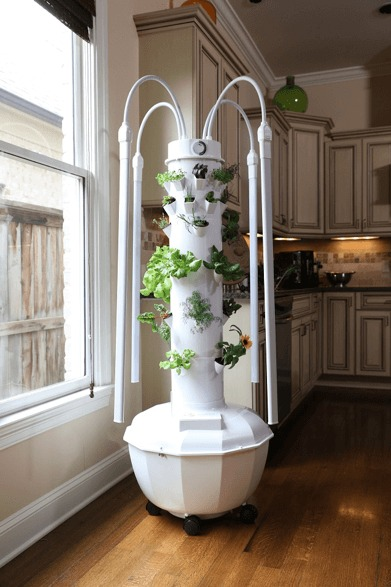
\includegraphics[width=0.3\linewidth]{plantacornerstone.jpeg}
            \\




}
}






    %=======================NOTES ENDS HERE===================%

    % bib stuff
    \nocite{*}
    \addtocontents{toc}{\protect\vspace{\beforebibskip}}
    \addcontentsline{toc}{section}{\refname}
    \bibliographystyle{plain}
    \bibliography{../Bibliography}
\end{document}
